\documentclass[12pt]{scrartcl}

\title{fLaCPGA - FPGA fLaC Decoder}
\subtitle{Requirements Analysis}
\author{Emmanuel Jacyna - 24227498}
\date{\today}

\usepackage[T1]{fontenc}
\usepackage[utf8]{inputenc}

\setkomafont{disposition}{\normalfont\bfseries}


\usepackage{graphicx}
\usepackage{tabularx}
\usepackage{float}
\usepackage{amsmath}
\usepackage{listings}
\bibliographystyle{unsrt}


\begin{document}
\pagestyle{myheadings}
\markright{Emmanuel Jacyna\hfill 24227498\hfill}
  \maketitle
  \tableofcontents
  
  \section*{Abstract}
  
  \section{Introduction}
  The goal of my final year project is to produce an implementation of a Free Lossless Audio Codec (henceforth, fLaC) decoder and encoder in Verilog for eventual use on an FPGA. fLaC is a lossless audio compression codec that is gaining popularity as a method of distributing high quality audio recordings and for compressing large audio archives\cite{findcite}. Whilst there are a number of software implementations of the fLaC encoder and decoder, there are no freely available hardware implementations. A hardware implementation would be of great use for a number of reasons. Many nations are now in the process of digitising large national audio archives. Audio archives require data to be compressed losslessly in order to preserve content in a form faithful to the original, however, uncompressed lossless data consumes large amounts of space. Currently, uncompressed formats such as WAVE and (BBWAVE?) are quite popular for audio archiving\cite{findcite}. Compressed audio has the major benefit of reducing space usage by up to half, doubling an archive's potential storage space. In order to convert large (terabytes) amounts of audio data to a compressed format, a lot of computing power is required. If a hardware decoder were available, it would both reduce encoding time and reduce power consumed by the encoding process. fLaC is also gaining popularity as a medium for portable audio players. The players are very sensitive to power consumption, a hardware implementation would be of great use in reducing the power load of the decoding process. Another potential use case of a hardware encoder would be in a recording studio. Instead of recording audio to an uncompressed format, high quality audio could be encoded in real time as it comes in.
  
  \section{Audio Compression Overview}
  Just as with general data compression, there are two main methodologies for compressing audio data, lossy and lossless. Lossy audio encoding most often includes techniques such as psychoacoustic compression, where sounds that humans cannot perceive or differentiate are removed from the audio. These techniques will not be the focus of this project. Lossless compression, by comparison, encodes audio perfectly, that is, the decoded audio is identical to the original input samples. Audio is still affected by problems such as quantisation noise and recording device noise.\\
  The main goal of any lossless compression algorithm is to remove redundancy from data, thereby reducing the amount of information needed to reproduce the data. Audio data is often highly redundant, samples of data that are close to each other will usually have very similar patterns, for example, samples of a clarinet playing the same note for a number of seconds will clearly have a similar spectral pattern over the period of time the note is held, thus offering redundancy to be exploited. The most popular method for lossless compression of audio data is to find an accurate model of the audio (a \textit{predictor}), find the error (often called \textit{residuals}) between the predictor and the true audio, then to encode the residuals using a variable bit length encoding in order to reduce the redundancy of the signal. The fLaC lossless audio compression algorithm borrows heavily from prior  work in lossless encoding including the Shorten algorithm\cite{shorten}, and the AudioPAK algorithm\cite{audiopak}. These algorithms use a technique called \textit{linear prediction} to produce their audio model, and use Rice encoding to perform the entropy encoding phase of the compression. The advantage of these algorithms is the ease with which they can be translated into hardware, as the linear prediction step consists of a number of multiplies and adds.
  
  \section{Requirements}
  \subsection{Documentation}
  A number of documents will be produced during this p
  \begin{itemize}
  \item Create a literature review
  \item Create final report
  \item Create a project description poster
  \item Encoder and Decoder documentation, including in code documentation (comments) and a user guide
  \end{itemize}
  
  \subsection{fLaC Decoder}
  \begin{itemize}
  \item Implement software fLaC decoder in C++
  \item Implement fLaC decoder in Verilog
  \item Develop Verilog testbenches for each module
  \item Test decoder on FPGA
  \item Produce audio output using Development Board DAC
  \end{itemize}
  
  \subsubsection{Metadata and Frame Decoding}
  \begin{figure}[H]
    \centering{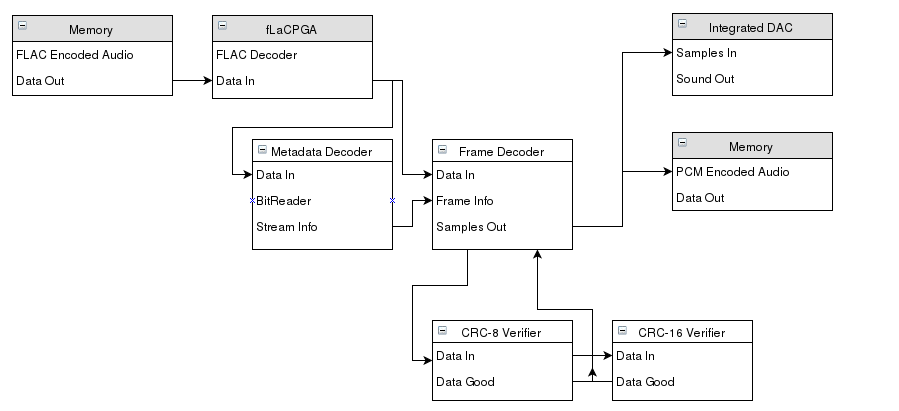
\includegraphics[scale=.8]{imgs/system_overview.png}}
    \caption{Overview of fLaCPGA Decoding System}
    \label{fig:system_overview}
  \end{figure}
  
  \begin{itemize}
  \item Decode fLaC Metadata stream
    \begin{itemize}
    \item Read and store variable bit length fields
    \item Read STREAMINFO metadata block
    \item Read and ignore all other metadata blocks
    \end{itemize}
  \item Decode fLaC Frame
    \begin{itemize}
    \item Read and store variable bit length fields
    \item Execute a CRC-8 check on the frame header
    \item Execute a CRC-16 check on the entire frame
    \item Decode each subframe
    \end{itemize}
  \end{itemize}
  
  \subsubsection{Subframe Decoding}
  \begin{figure}[H]
    \centering{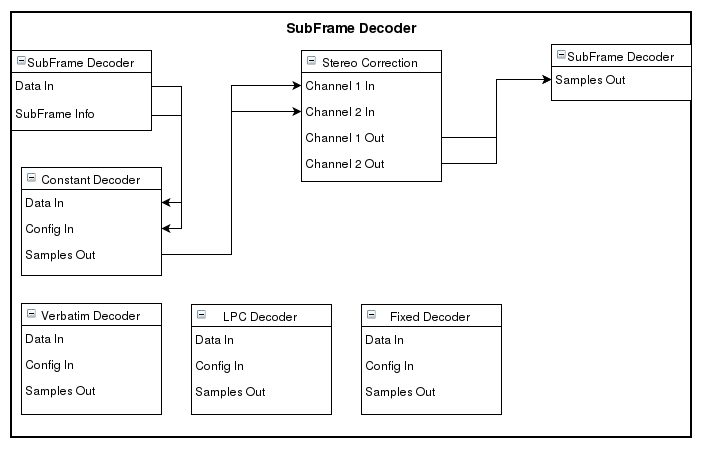
\includegraphics[scale=.8]{imgs/subframe_decoder_overview.png}}
    \caption{Overview of fLaCPGA Subframe Decoding System}
    \label{fig:subframe_overview}
  \end{figure}
  
  \begin{itemize}
  \item Decode fLaC Subframe
    \begin{itemize}
    \item Decode Constant encoded subframe
    \item Decode Verbatim encoded subframe
    \item Decode Fixed encoded subframe
    \item Decode LPC Encoded subframe
    \item Correct stereo decorrelation
    \end{itemize}
  \end{itemize}
  
  \subsubsection{LPC and Fixed Decoding}
  \begin{figure}[H]
    \centering{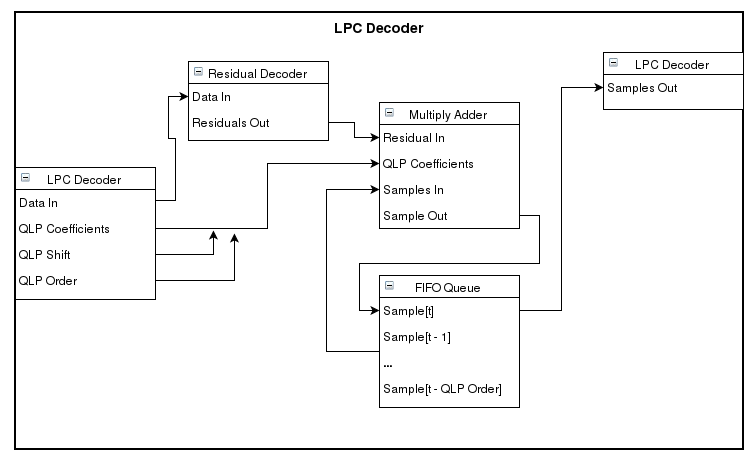
\includegraphics[scale=.8]{imgs/LPC_Decoder_Overview.png}}
    \caption{Overview of fLaCPGA LPC Subframe Decoding System}
    \label{fig:LPC_overview}
  \end{figure}
  \begin{itemize}
  \item Decode LPC and Fixed Subframes
    \begin{itemize}
    \item Read and store variable bit length fields
    \item Decode fLaC Specification residual
      \begin{itemize}
      \item Decode rice encoded variable length bit stream
      \end{itemize}
    \item Perform LPC decoding using residuals and predictor coefficients
    \end {itemize}
  \end{itemize}
  
  \subsection{fLaC Encoder}
  \begin{itemize}
  \item Implement software fLaC encoder in C++
  \item Implement fLaC encoder in Verilog
  \item Develop Verilog testbenches for each module
  \item Test encoder on FPGA
  \end{itemize}
  
  \section{Conclusion}

  \bibliography{references}
  
\end{document}
